%This file has descriptions of mom. and (outgoing) energy-loss corrections.
% Check the pass2 mom. cor. routine with a link available at the following wiki page:
%      https://clasweb.jlab.org/rungroups/eg4/wiki/index.php/Momentum_Correction_(Pass2)
%  or at https://www.jlab.org/Hall-B//secure/eg4/adhikari/myHomeLinked/MyHm/LinkedFiles/momCorPass2.h


\subsection{Momentum Correction}
Different DC related factors contribute to the biggest part of the systematic deviations of particle momenta as reconstructed by RECSIS. The drift chambers could be misaligned relative to their nominal positions or the survey results that is used by RECSIS could be inaccurate or out-of-date. The effects of physical deformations (due to thermal and stress distortions) of the chamber including wire-sag, incorrect wire positions may not have bee incorporated properly. The torus field map used by the reconstruction software may not have been accurate and complete enough \cite{e6momcor_cn}. Effects on angles \th and \ph due to these contributions are already factored in the tracking correction described earlier. However, a separate method is developed to correct for the effect on the magnitude $p$ of the momentum. This $p$-correction methods picks up and builds on some of the ideas outlined in the CLAS-NOTE 2003-005 \cite{e6momcor_cn}.

\subsubsection{Procedure to determine the first 11 parameters}
\label{pCorFit1}
The procedure involved dividing the covered kinematic space into a number of bins, finding in them the magnitude of shifts of the inclusive 
elastic peaks w.r.t. the expected position and use that to fit to a function to get an analytical expression for the correction. The 
following angular bins were used:
\begin{itemize}
\item Six $\theta_{dc1}$ bins: (0,8),(8,10),(10,12),(12,15),(15,20),(20,30) degrees
\item Five $\phi_{dc1}$ bins: (-10,-6),(-6,-2), (-2,2), (2,6), (6,10) degrees 
\end{itemize}
where the angles used are the ones measured at the first drift chamber and $\phi_{dc1}$ is measured w.r.t the sector mid-plane (thus the 
maximum range allowed is (-30.0,30.0)).
  
\begin{eqnarray}
\label{eqElasticEprime}
E'_{elastic} = \frac{E_{beam}}{1+\frac{2E_{beam}}{M_p}sin^2(\theta_e/2)}
\end{eqnarray}

%\textcolor{red}{To be expanded later on.}

In each of these kinematic bins, the quantity $\Delta E = E'_{elastic} - p$ (see Eq. \ref{eqElasticEprime}) is histogrammed for both NH$_3$ and $^{12}$C data separately. Next, the carbon histogram is cross-normalized with the ammonia histogram (by comparing the two in the region left to the quasi-elastic peak) and subtracted from the latter one to remove the nuclear background. The difference gives  histograms for the elastic events (as shown by the dashed green histogram in Fig. \ref{sec6dEall}). A Gaussian fit to the extracted elastic histogram gives the position and width of the distribution. The offset or shift of average position of the peak with respect to the expected $\Delta E = 0$ gives us the needed correction on energy $E \approx p$ for the electron. This process is repeated for all of the bins listed above and the corresponding $\Delta E$ offsets or the corrections are determined for each of them. Additionally, $\Delta E$ distributions using $^{15}N$ nuclear mass in calculating $E'_{elastic}$ are also made and off-sets in the corresponding elastic peaks are also recorded whenever possible (particularly from the lower \th bins from low beam energy data where the nuclear-elastic and quasi-elastic peaks are well separated).
% https://clasweb.jlab.org/rungroups/eg4/wiki/index.php/Momentum_Correction_(Pass2)#6.2F23-30.2F15
%https://www.jlab.org/Hall-B//secure/eg4/adhikari/Corrections/Mcor/Pass2/IncMcor/GfOp/elasticPeaksFromNH3wdWoCorEi0.gif
%https://www.jlab.org/Hall-B//secure/eg4/adhikari/Corrections/Mcor/Pass2/IncMcor/GfOp/elasticPeaksFromNH3wdWoCorEi0mN15.gif
Finally, these values of corrections for different average values of $\theta_{dc1}$ and $\phi_{dc1}$ are fit to Eq. \ref{eqPCor} (which is based on similar work done for EG1b analysis\cite{nGuler_th})
and using the method of \chisq-minimization in order to determine the values of the 11 fit parameters.


\begin{eqnarray}
\label{eqPCor}
\frac{\Delta p}{p} = Pcorr1 + Pcorr2 + PatchCorr
\end{eqnarray}
where, $\frac{\Delta p}{p}$ is the ratio of the correction ($\Delta p$) to the magnitude ($p$) of the momentum and 
\begin{eqnarray}
\label{eqPCor1}
%\frac{\Delta p}{p} = ((E+F\phi)\frac{cos\theta}{sin\phi} + (G+H\phi)sin\theta)\frac{p}{qB_{torus}}  %Smallest normal sized parentheses
%\frac{\Delta p}{p} = \big( (E+F\phi)\frac{cos\theta}{sin\phi} + (G+H\phi)sin\theta   \big) \frac{p}{qB_{torus}} % same as above
%\frac{\Delta p}{p} = \Big( (E+F\phi)\frac{cos\theta}{sin\phi} + (G+H\phi)sin\theta   \Big) \frac{p}{qB_{torus}} %Bigger parentheses
%\frac{\Delta p}{p} = \bigg( (E+F\phi)\frac{cos\theta}{sin\phi} + (G+H\phi)sin\theta   \bigg) \frac{p}{qB_{torus}} %Bigger parentheses
Pcorr1 = \left( (E+F\phi)\frac{cos\theta}{sin\phi} + (G+H\phi)sin\theta   \right) \frac{p}{qB_{torus}} %Biggest parentheses
\end{eqnarray}


\begin{eqnarray}
\label{eqPCor2}
%\frac{\Delta p}{p} = (J cos\theta + K sin\theta) + (M cos\theta+N sin\theta)\phi
Pcorr2 = (J cos\theta + K sin\theta) + (M cos\theta+N sin\theta)\phi
\end{eqnarray}

\begin{eqnarray}
\label{eqPatchCor}
PatchCorr = 0.02\left(P + (Q + R\frac{\phi_{deg}}{30^\circ})(\frac{10^\circ}{\theta_{deg}})^3 \right) 
\end{eqnarray}

The quantity $B_{tor}$ stands for $\int{B_{\perp}dl}$ along the track length multiplied by the speed of light in the units 
of m/ns (c = 0.29979 m/ns) and is given by

\begin{eqnarray}
\label{eqBtor1}
%B_{tor} = 0.76 \frac{I_{tor}sin^2(4\theta)}{3375\theta/rad} \quad  for \quad  \theta < \frac{\pi}{8} %itallic text 'for'
B_{tor} = 0.76 \frac{I_{tor}sin^2(4\theta)}{3375\theta/rad} \quad  \rm{for} \quad  \theta < \frac{\pi}{8} %Roman (no itallic)
%B_{tor} = 0.76 \frac{I_{tor}sin^2(4\theta)}{3375\theta/rad} \quad  \mathrm{for} \quad  \theta < \frac{\pi}{8} %Roman (no itallic)
%B_{tor} = 0.76 \frac{I_{tor}sin^2(4\theta)}{3375\theta/rad} \quad  \textrm{for} \quad  \theta < \frac{\pi}{8} %Roman (no itallic)
\end{eqnarray}

\begin{eqnarray}
\label{eqBtor2}
B_{tor} = 0.76 \frac{I_{tor}}{3375\theta/rad}  \quad  \textrm{for}  \quad  \theta > \frac{\pi}{8}
\end{eqnarray}

In all these equations, sector number, $\theta$, $\phi$, $\theta_{deg}$, and $\phi_{deg}$ come from the angle information measured at DC1. The direction cosine variables tl1\_cx, tl1\_cy, tl1\_cz (from pass1 ntuples) are used to derive these quantities. C++ standard functions acos() and atan2() are used to evaluate $\theta$, $\phi$ (w.r.t the sector mid plane). %(One should take an extra care of the fact that the function atan2() gives the values of azimuthal angle $\phi$ between -$\pi$ to +$\pi$.) %SEK cor 12/4/13



These total of eleven unknown parameters were determined by fitting above mentioned momentum offsets (in combination with ionization energy loss correction for electrons (see Sec.\ref{secElossCor} below)) to the correction function given by the Eq. \ref{eqPCor}.




\begin{figure}[H]%[ht] 
%\centerline{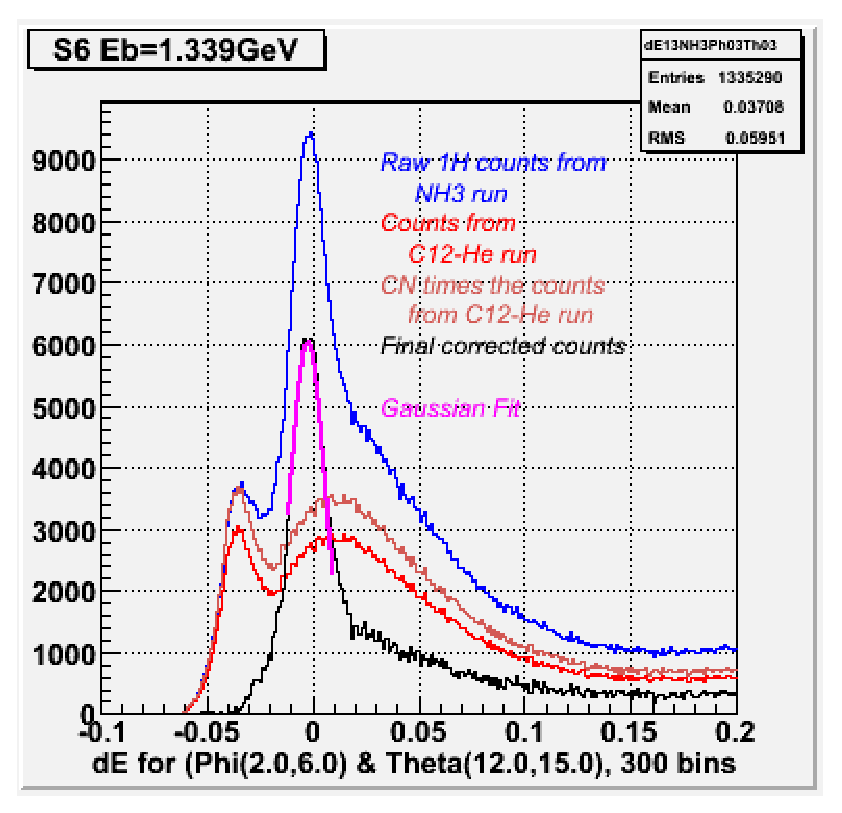
\epsfig{height=10cm,width=15cm,file=chap7KineCor/figures/HiStatNH3_1339_3_o1.eps}}
%\caption[The world data for the proton form factor ratio $\mu_p\frac{G_E}{G_M}$ extracted using Rosenbluth separations.]{The world 
%data for the proton form factor ratio $\mu_p\frac{G_E}{G_M}$ extracted using Rosenbluth separations ~\cite{qatan_th}.}
%\caption[Background removal from $\Delta E$]{Plot showing background removal from the $\Delta E$ counts (shown in blue) from $NH_3$ data 
%(by subtracting cross-normalized counts from $^{12}C$ data (shown in red)) to separate the elastic peak (black) in one of the kinematic bins, 
%thereby getting the momentum offset for that bin.}
\centering
  %\leavevmode 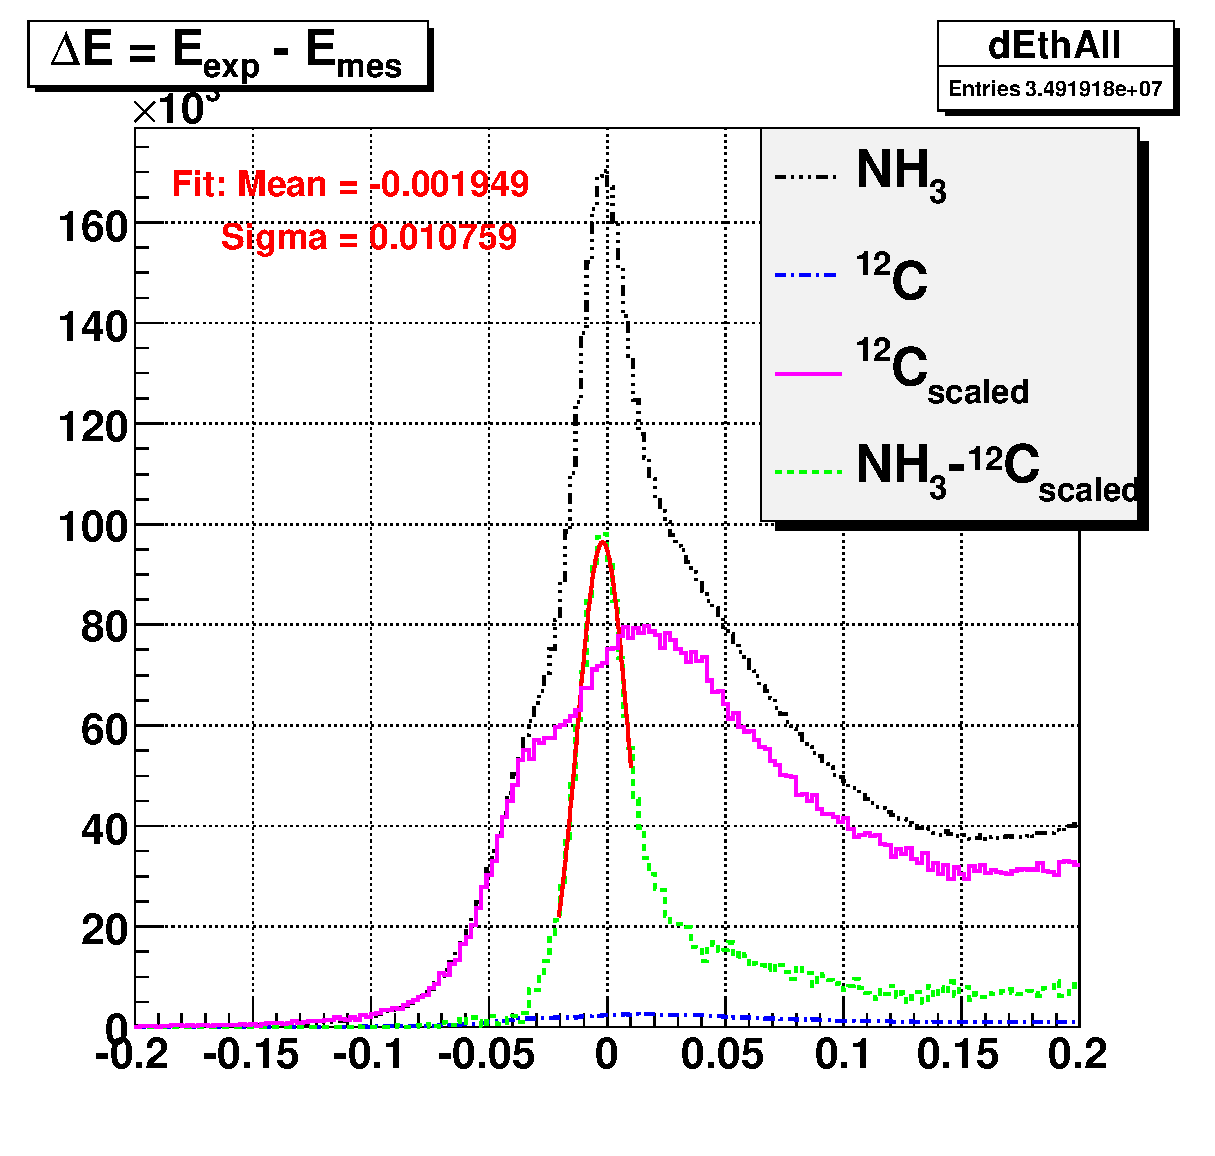
\includegraphics[width=0.8\textwidth]{chap4simul/DcSmear/dE_elastProdEb3.eps} 
  \leavevmode 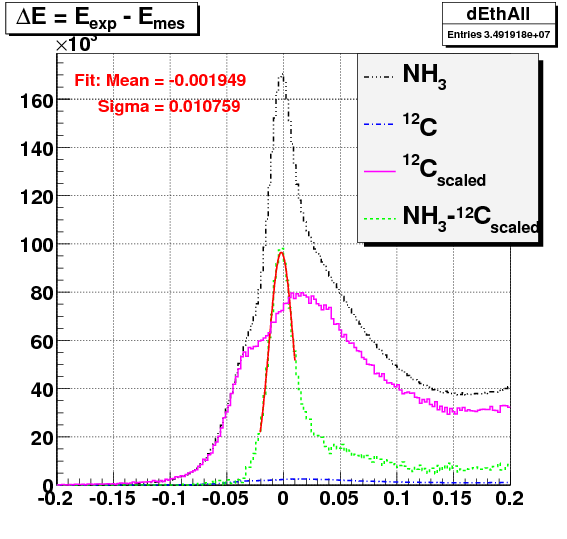
\includegraphics[width=0.8\textwidth]{figuresEG4/FigKineCor/dE_elastProdEb3.png} 
%\centerline{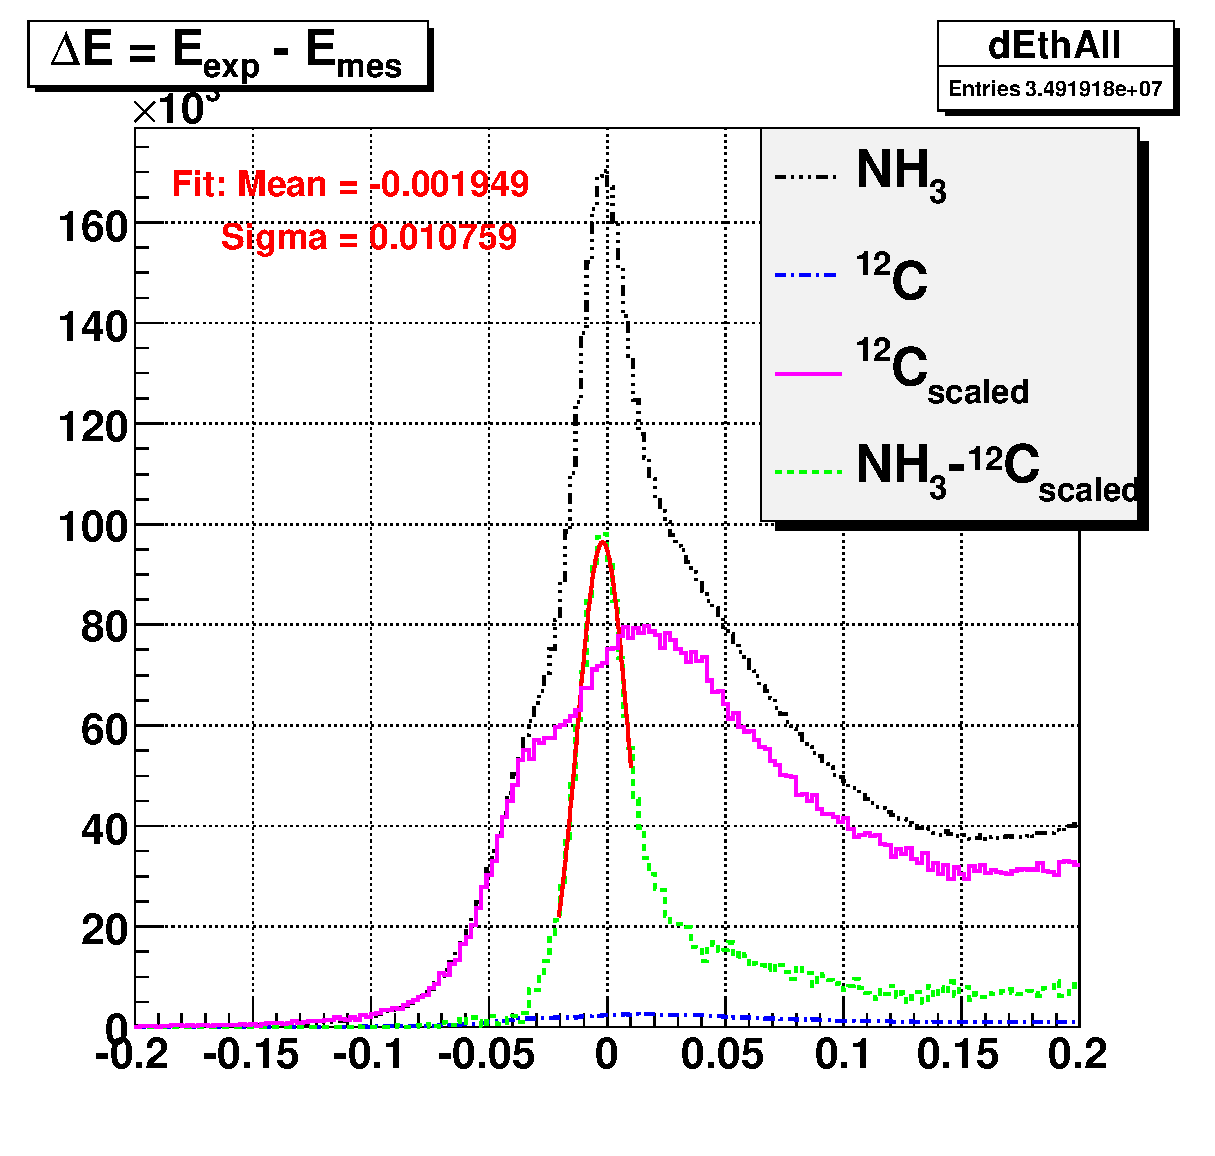
\epsfig{height=10cm,width=15cm,file=chap4simul/DcSmear/dE_elastProdEb3.eps}}
 % \caption[Background subtraction to get elastic peak]{Histograms illustrating the extraction of elastic peak for 2.3 GeV by using 
%carbon-12 data for background removal from the total-cross section (all good electrons with $\theta>7$ used).}
  \caption[Background removal from $\Delta E$]{Plots showing background removal from the $\Delta E$ counts from NH$_3$ 
(shown by ``NH$_3$'' line) data (by subtracting cross-normalized counts from $^{12}$C data (shown by ``$^{12}$C$_{scaled}$'' 
line)) to separate the elastic peak (shown by ``NH$_3$ - $^{12}$C$_{scaled}$'' line) in one of the kinematic bins, thereby 
getting the momentum offset for that bin.}
%^{235}_{92}U an example of how an Uranium isotope symbol in Chemistry written with the Latex %kp: April 04, 2010
\label{sec6dEall}
\end{figure}


\begin{figure}[H]%[ht] 
\centering
  \leavevmode 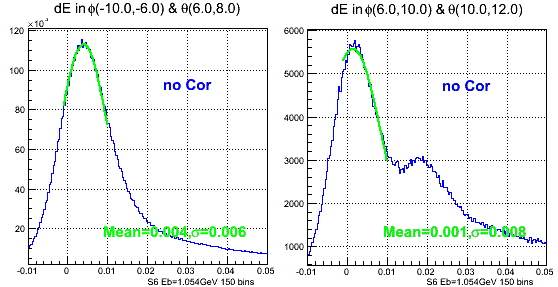
\includegraphics[width=0.8\textwidth]{figuresEG4/FigKineCor/elasticPeaksFromNH3wdWoCorEi0mN15gausCropped.png} 
  \caption[Nuclear elastic peak fron $^{15}$N target]{Nuclear elastic peaks fron $^{15}$N target and the Gaussian fits in two
of many kinematic bins as seen in $\Delta E = E'_{elastic} - p$ distributions from NH$_3$ data before the momentum corrections.
In this case $E'_{elastic}$ is evaluated using known mass of $^{15}$N in Eq. \ref{eqElasticEprime}.
In the second plot, the proton elastic peak is also visible. Ideally, after all the corrections, the nuclear elastic peak is 
expected to be centered at zero. But, as is obvious from these figures, these peaks show offsets. These offsets (given
by the mean values of the Gaussian fits) are collected from those bins in which the nuclear elastic peaks are very well
separated (particularly the first few angular bins) and used in the $\chi^2$-minimization along with all the offsets of
elastic peaks (see Fig. \ref{sec6dEall})}
\label{sec6dEnucElastEbi0}
\end{figure}



\begin{comment}
\begin{figure}[htpb] %ht, htpb (p - float, b = bottom, h=? t = top)
%\centerline{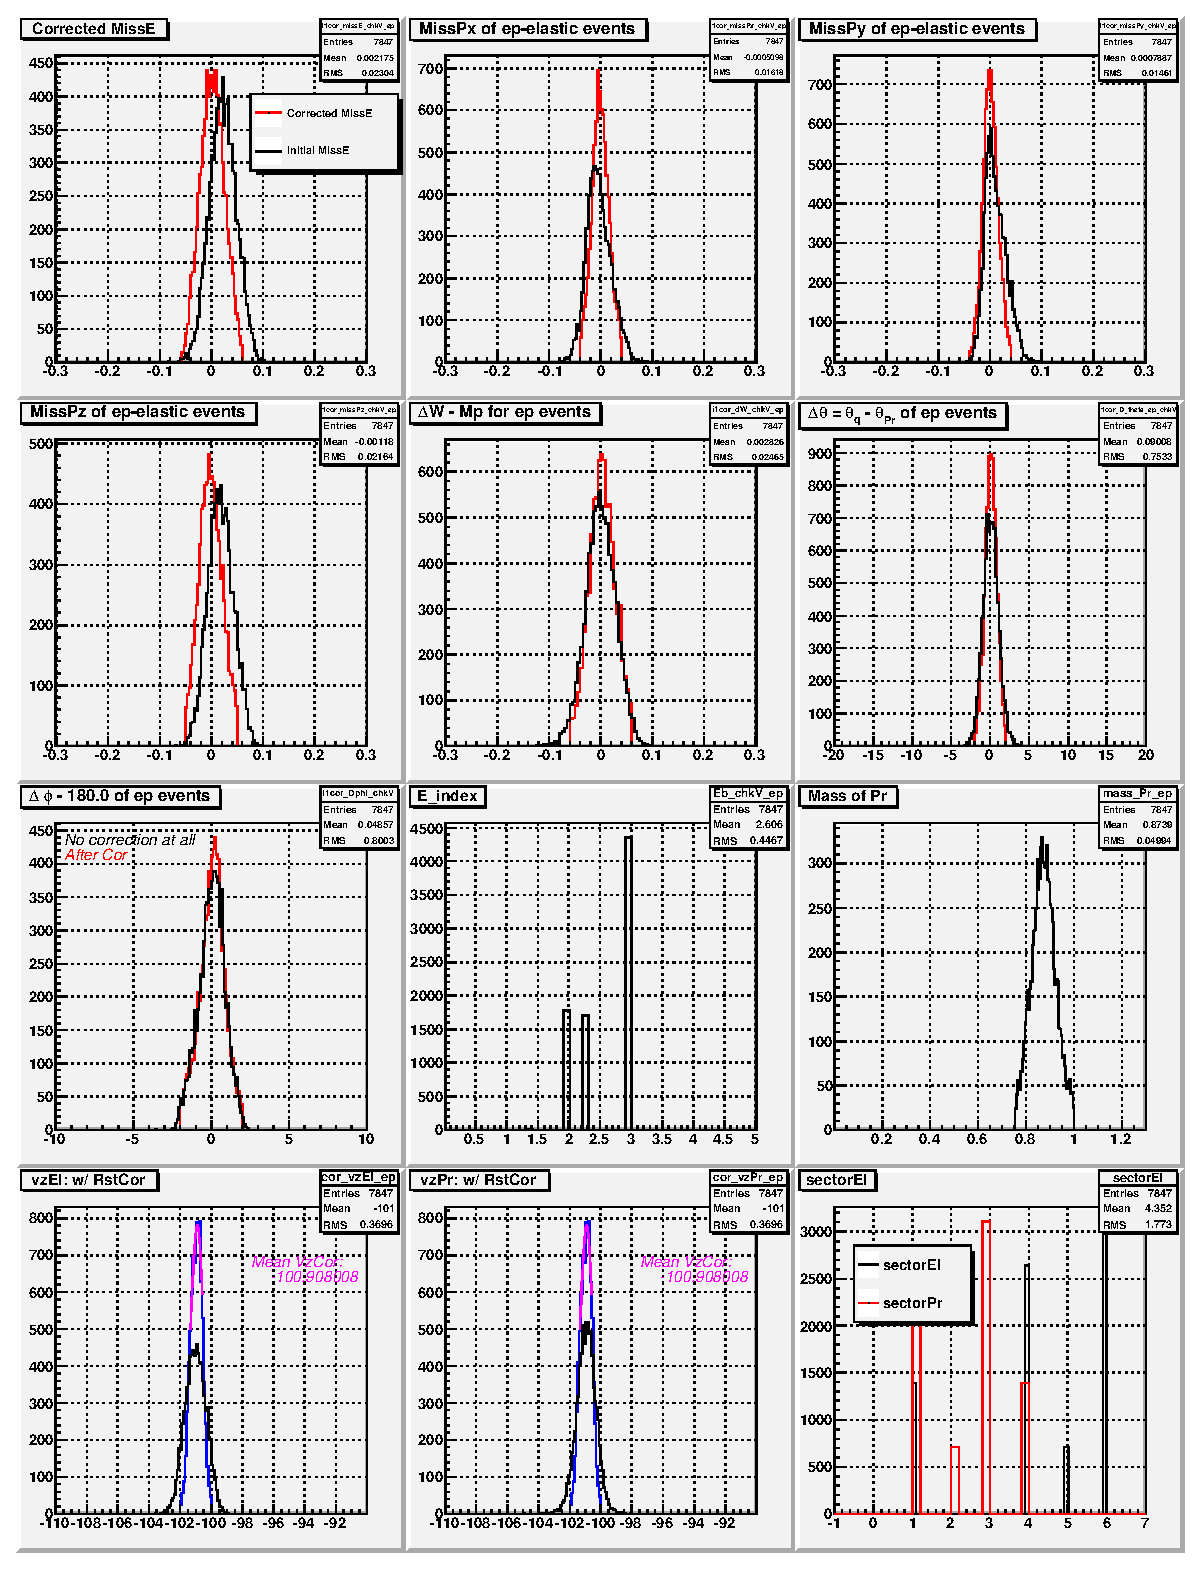
\epsfig{height=20cm,width=15cm,file=chap7KineCor/figures/ep_evntsChkMcor.eps}}
\centering
% \leavevmode 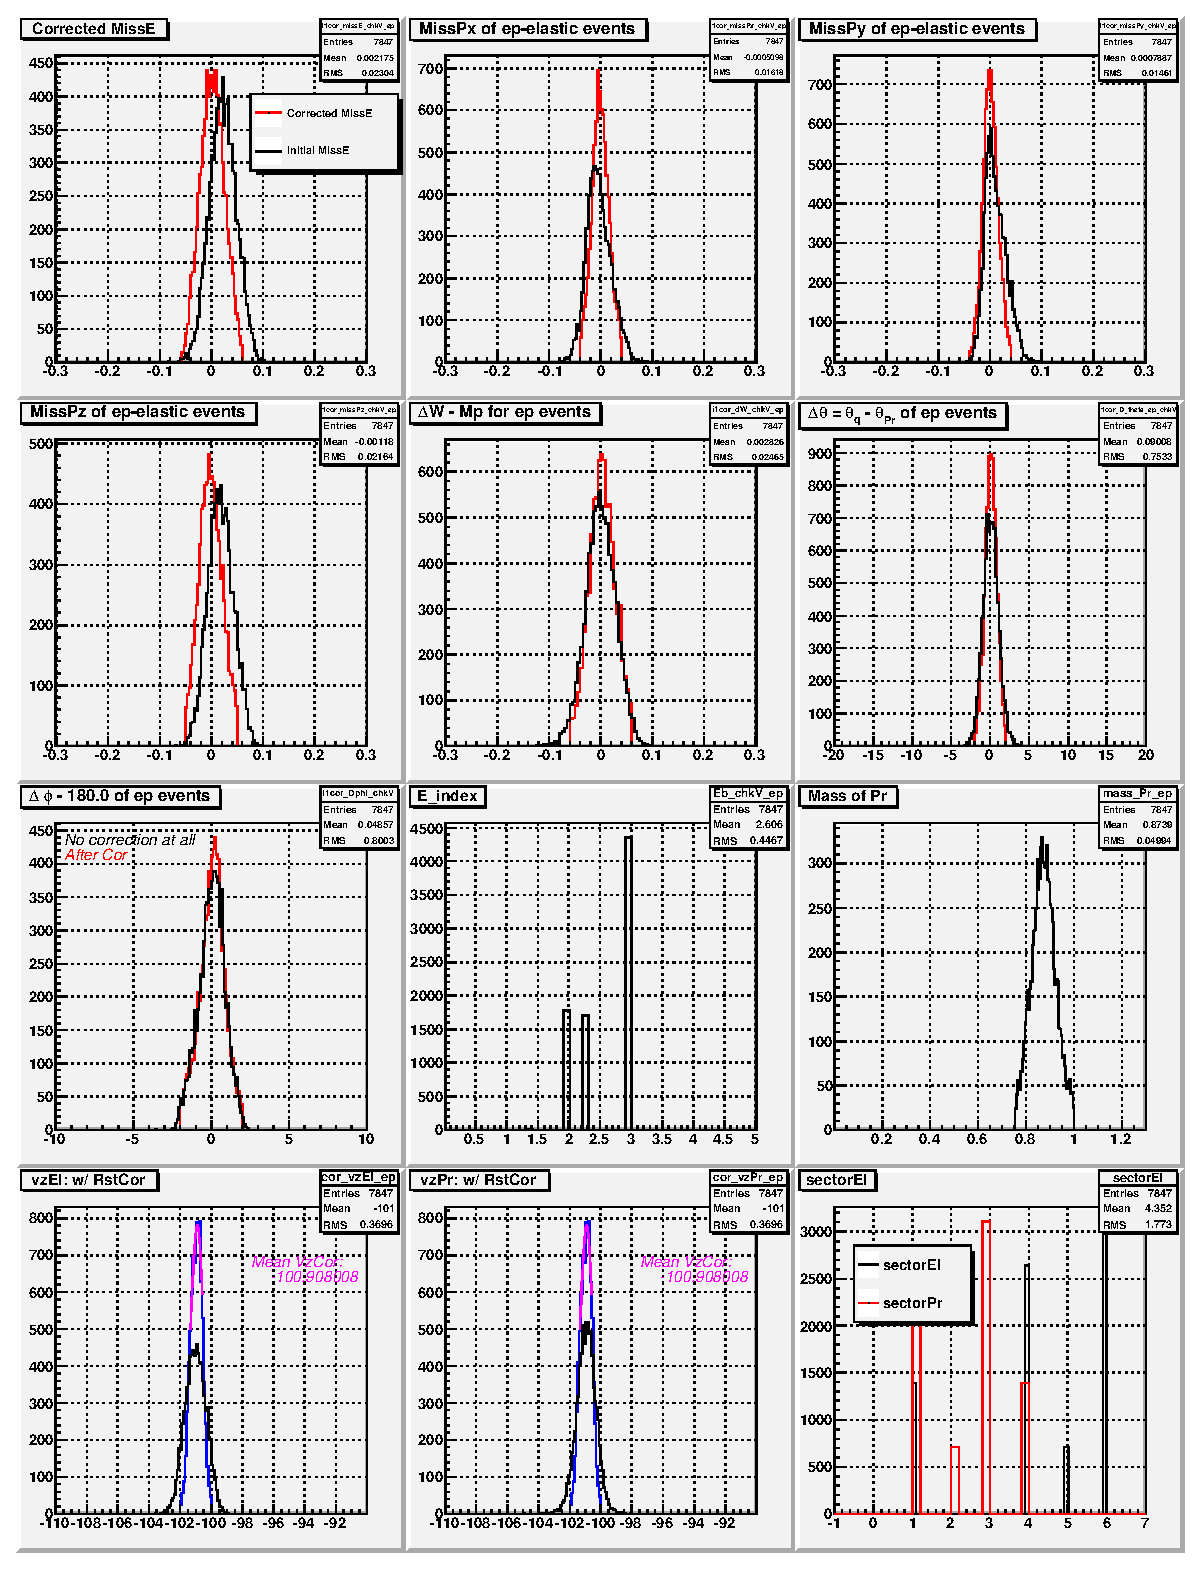
\includegraphics[width=0.85\textwidth]{chap7KineCor/figures/ep_evntsChkMcor.eps} %Used till 11/30/13
%\caption[Effects of corrections ep-elastic events]{Effects of kinematic corrections on ep-elastic events. The first 6 panels 
%show distributions (before ({\bf black}) and after (\textcolor{red}{{\bf red}}) the corrections) of the missing energy, missing 
%(X,Y,Z) components of momenta, $\Delta W = W - M_p$, and $\Delta \theta = \theta_q - \theta_p$, where $\theta_q$ and $\theta_p$ 
%are the expected and measured angles of the recoil proton (or the exchanged virtual photon). The 7th plot is for $\Delta \phi - 180.0$, 
%where $\Delta \phi = \phi_e - \phi_p$. The 10th and 11th plots show the Z-vertex distributions of electrons and protons before 
%({\bf black}) and after (\textcolor{blue}{{\bf blue}}) the corrections.} %Used till 11/30/13
 %\leavevmode 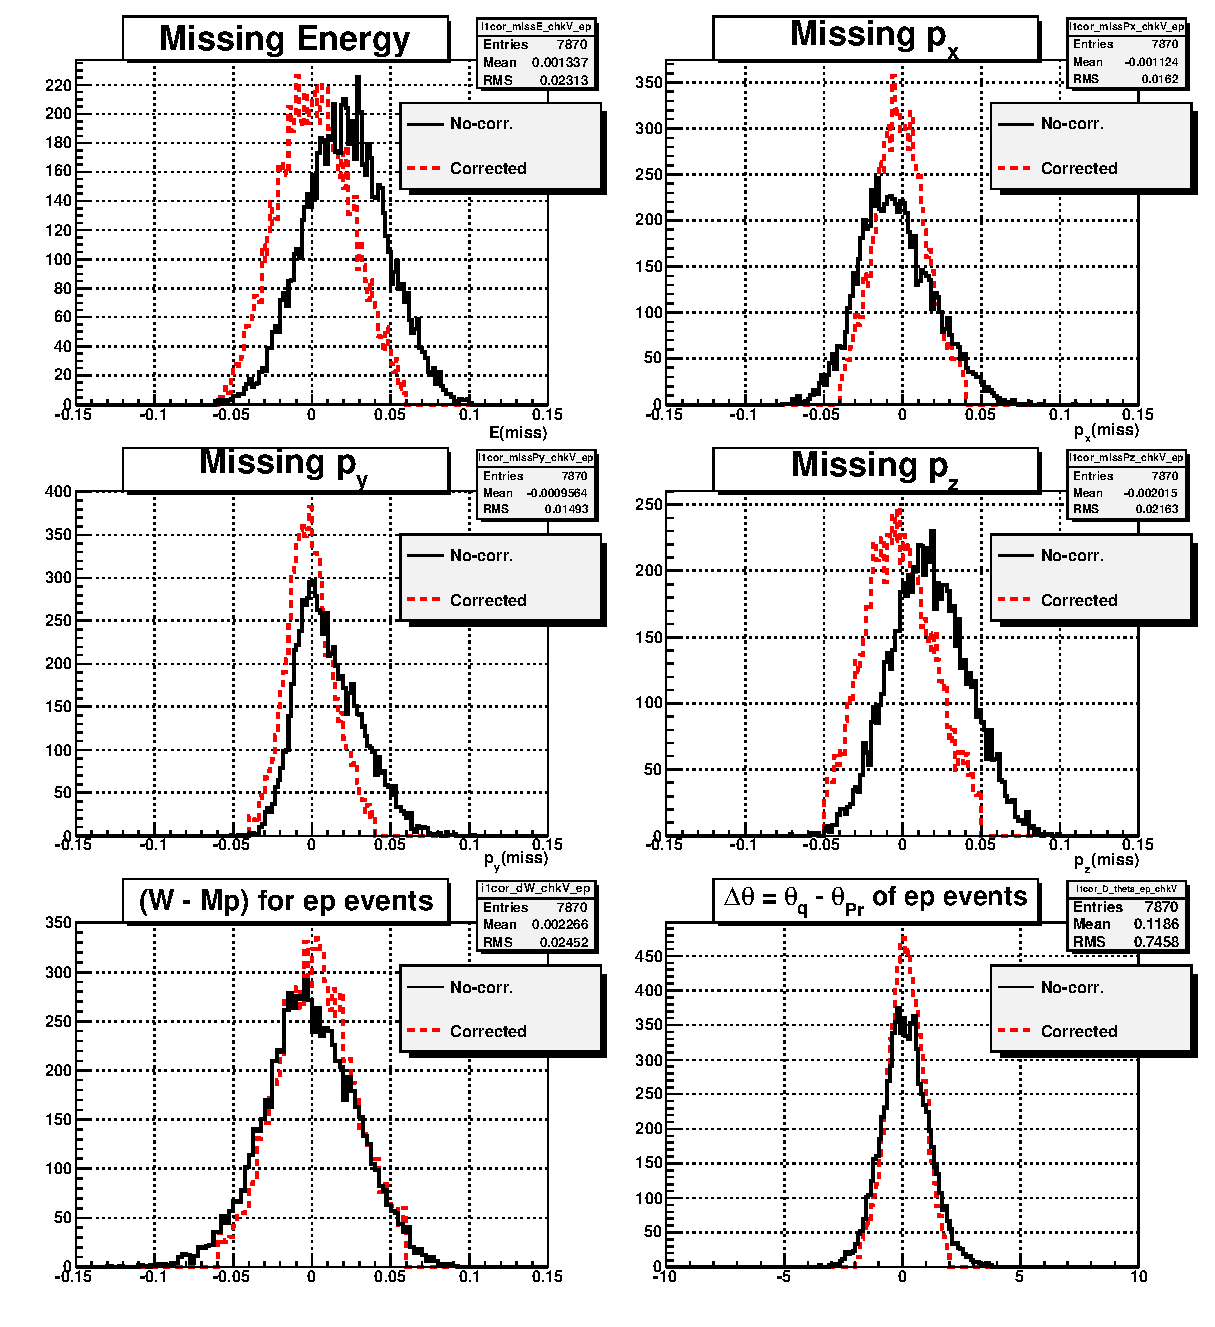
\includegraphics[width=1.0\textwidth]{chap7KineCor/figures/ep_evntsChkMcor2.eps} 
 \leavevmode 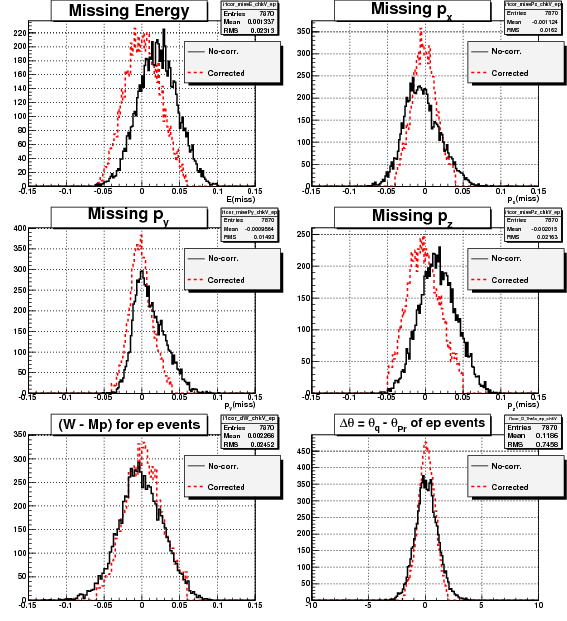
\includegraphics[width=1.0\textwidth]{figuresEG4/FigKineCor/ep_evntsChkMcor2.png} 
\caption[Effects of corrections on ep-elastic events]{Effects of kinematic corrections on ep-elastic events. In the 6 panels the 
distributions of missing energy, missing momentum components ($p_x$, $p_y$, and $p_z$), the difference $\Delta W = W-M_p$ and 
$\Delta \theta = \theta_q - \theta_{p}$ of ep-elastic events respectively. The distributions before the corrections are shown 
by {\bf black continuous} lines and the ones after the corrections are shown by the \textcolor{red}{{\bf red dotted}} lines. 
Here, $M_p$ is the proton mass in GeV. Likewise, $\theta_q$ and $\theta_p$ are the expected and measured angles of the recoil 
proton (or the exchanged virtual photon) respectively. }
\label{fig:epElastic}
\end{figure}
\end{comment}




%\subsection{Correction for the Outgoing Energy Loss due to Ionization}
\subsection{Outgoing Ionization Loss Correction}
\label{secElossCor}
 
%    \sqrt[root]{arg} The \sqrt command produces the square root of its argument. The optional argument, root, determines what root 
%    to produce, i.e., the cube root of x+y  would be typed as  $\sqrt[3]{x+y}$
In addition to the corrections described above, the energy (E) of each of the particles is corrected for the outgoing ionization loss by adding an estimation of ionization loss as follows: $E_{cor} = E + \Delta E $ with $\Delta E = \frac{dE}{dX}\tau$ % $\Delta E = (\frac{\Delta E/\Delta X}{1000.0})gm$,
where the factor $\tau$ is the total effective mass thickness traversed by the particle and
\begin{subequations}
\begin{eqnarray}
\label{eqElossEl}
%\Delta E/ \Delta X = 2.8 ~MeV \quad \rm{for ~electrons}
dE/dX \approx 2.8 ~\rm{MeV/(g ~cm}^{-2}\rm{)} \quad \rm{for ~electrons}
\end{eqnarray}
and, for hadrons \cite{leo1994techniques}
\begin{eqnarray}
\label{eqElossHad}
%%%if( mass < 0.01) DEDX = 2.8;    else DEDX = 0.307 * ( 0.5 / Beta2 ) * ( log( 2. * 511000.0 * Beta2 * ( Gamma2 / 90. ) ) - Beta2 );
%%%\Delta E/ \Delta X = 0.307 (\frac{ 0.5}{ \beta^2}) \left( log\bigg( 2.0( 511000.0 \beta^2) (\frac{ \gamma^2}{ 90.0} ) \bigg) - \beta^2 \right);
%%%\Delta E/ \Delta X = 0.307 (\frac{ 0.5}{ \beta^2}) \left( ln\bigg( 2.0( 511000.0 \beta^2) (\frac{ \gamma^2}{ 90.0} ) \bigg) - \beta^2 \right) ~MeV ~\rm{for ~hadrons} 
%\Delta E/ \Delta X = 0.307 \times \frac{ 0.5}{ \beta^2} \left( ln\bigg( 2.0 \times 511.0 \frac{\beta^2 \gamma^2}{ 0.090} \bigg) - \beta^2 \right) ~MeV 
dE/dX \approx 0.307 \times \frac{ 0.5}{ \beta^2} \left( ln\bigg( 2.0 \times 511.0 \frac{\beta^2 \gamma^2}{ 0.090} \bigg) - \beta^2 \right) \rm{~MeV} 
\end{eqnarray}
\end{subequations}
which is an approximation of the Bethe-Block formula \cite{leo1994techniques}: % (Eq.(\ref{eqBetheBlock})).

\begin{eqnarray}
\label{eqBetheBlock}
-\frac{1}{\rho} \frac{dE}{dx} = 4\pi N_a r_e^2 m_e c^2 \frac{Z}{A} \frac{1}{\beta^2} \left( ln\bigg( \frac{2m_ec^2\gamma^2\beta^2}{I} \bigg) - \beta^2 \right) 
\end{eqnarray}
%And, the factor '$\tau$' is the total effective mass thickness traversed by the particle. 
This quantity is calculated as follows:
\begin{itemize}
\item $\tau = \tau_{\parallel}/cos\theta$ \quad if $\theta <= \pi/4$
\item $\tau = \tau_{\parallel}/cos(\pi/4)$ \quad if $\theta > \pi/4$    %SEK comment:  I don't understand. leave out! Why not \tau = r/sin \theta    (anyway \theta > \pi/4 is never true!
\end{itemize}
where $\tau_{\parallel}$ is calculated as:
\begin{itemize}
\item $\tau_{\parallel} = \Delta z \times 0.6 + 0.4$ \quad if $\Delta z > 0.0 $ and $\Delta z < 1.0 $
\item $\tau_{\parallel} = 0.6 + 0.4$ \quad if $\Delta z \geq  1.0$
\item $\tau_{\parallel} = 0.4$ \quad if $\Delta z \leq  0.0$
%\item $\tau_{\parallel} = 0.75$ \quad if otherwise
\end{itemize}
with $\Delta z = z_{target\_center} - z_{ave} + L_{target}/2 = (-101.0$ cm $ - z_{ave} + 0.5)$ cm being the physical distance (along the target length) traveled by the particle through the polarized target material (e.g. the EG4 ND$_3$ target has length 1.0 cm and is positioned at z = -101.0 cm). The factor 0.6 is the effective mass thickness of ND$_3$ (density of ND$_3$ ($\sim 1 ~g/cm^3$) %(e.g. one of the EG4 NH$_3$ (ND$_3$ too) target has length 1.0 cm and is positioned at z = -101.0 cm). The factor 0.6 is the effective mass thickness of NH$_3$ (density of NH$_3$ ($\sim 1 ~g/cm^3$) 
multiplied by the packing fraction which is roughly 0.6  \cite{rfersch_th}, whereas 0.4 is the sum of the mass thicknesses of He ($\sim 0.3$) and that of window foils ($\sim 0.1$) \cite{nGuler_th}. %In fact these numbers were for NH3 targets and were decided when our own values for PFs were not available which are now at about 0.7 (I believe, this won't make things much different, may be systematic study has to be done. 12/5/13)


% double zcenter    = -101.0; //-55.1;//#ignore
%  double \Delta z = zcenter - zave + 0.5;//#ignore
%  //kp:  \Delta z is the fraction of the distance the particle travelled i.e. \Delta z = (zave - zcenter + 0.5)/Lt  (Lt = target length = 1.0 for EG1B)
%  //     (denoted by delta_z in Nevzat's thesis), also in thesis, the order of zave -zcenter is wrong.
%  double E = sqrt(p*p + mass*mass);
%  double fbeta = p/E;  double Beta2 = fbeta * fbeta; double Gamma2 = 1.0 / ( 1.0 - Beta2 );  
    
%    if( ( \Delta z <= 1.0 ) && ( \Delta z >= 0.0 ) )  \tau = \Delta z * 0.6 + 0.4;
%    //kp: I think \tau is total effective mass thickness traversed by the particle
%    //    The factor 0.6 is effective mass thickness of NH$_3$ (density of NH$_3$ (about 1 g/cm^3) multiplied by the packing fraction which is 
%    //    roughly 0.6; See R. Fersch's thesis at page 215) and 0.4 is the sum of 0.3 and 0.1 where
%    //    0.4 is for mass thickness of He and 0.1 for that of window foils (see Nevzat's thesis, page 158)

%    else if( \Delta z >= 1.0 )  \tau = 0.6 + 0.4;
%    else if( \Delta z <= 0.0 )  \tau = 0.4;
%    else  \tau = 0.75;
%   //Ignore all above lines with '#ignore' and use '\tau = 0.75' for all cases for a reasonable approximation (Dr. Kuhn)
    
%    if( theta * rad2deg <= 45. ) \tau = \tau / cos( theta );
%    else  \tau = \tau / cos( 45. * deg2rad );

Using the ionization loss corrected energy and the rest mass of the particle, momentum is recalculated as $p_{cor} = \sqrt{E^2_{cor}-m^2}$ 
(where $m$ is the mass of the particle). Finally, this new p is used along with the previously corrected angles to evaluate the three 
cartesian components $p_x$, $p_y$ and $p_z$ of the momentum.




\begin{figure}[htpb] %ht, htpb (p - float, b = bottom, h=? t = top)
%\centerline{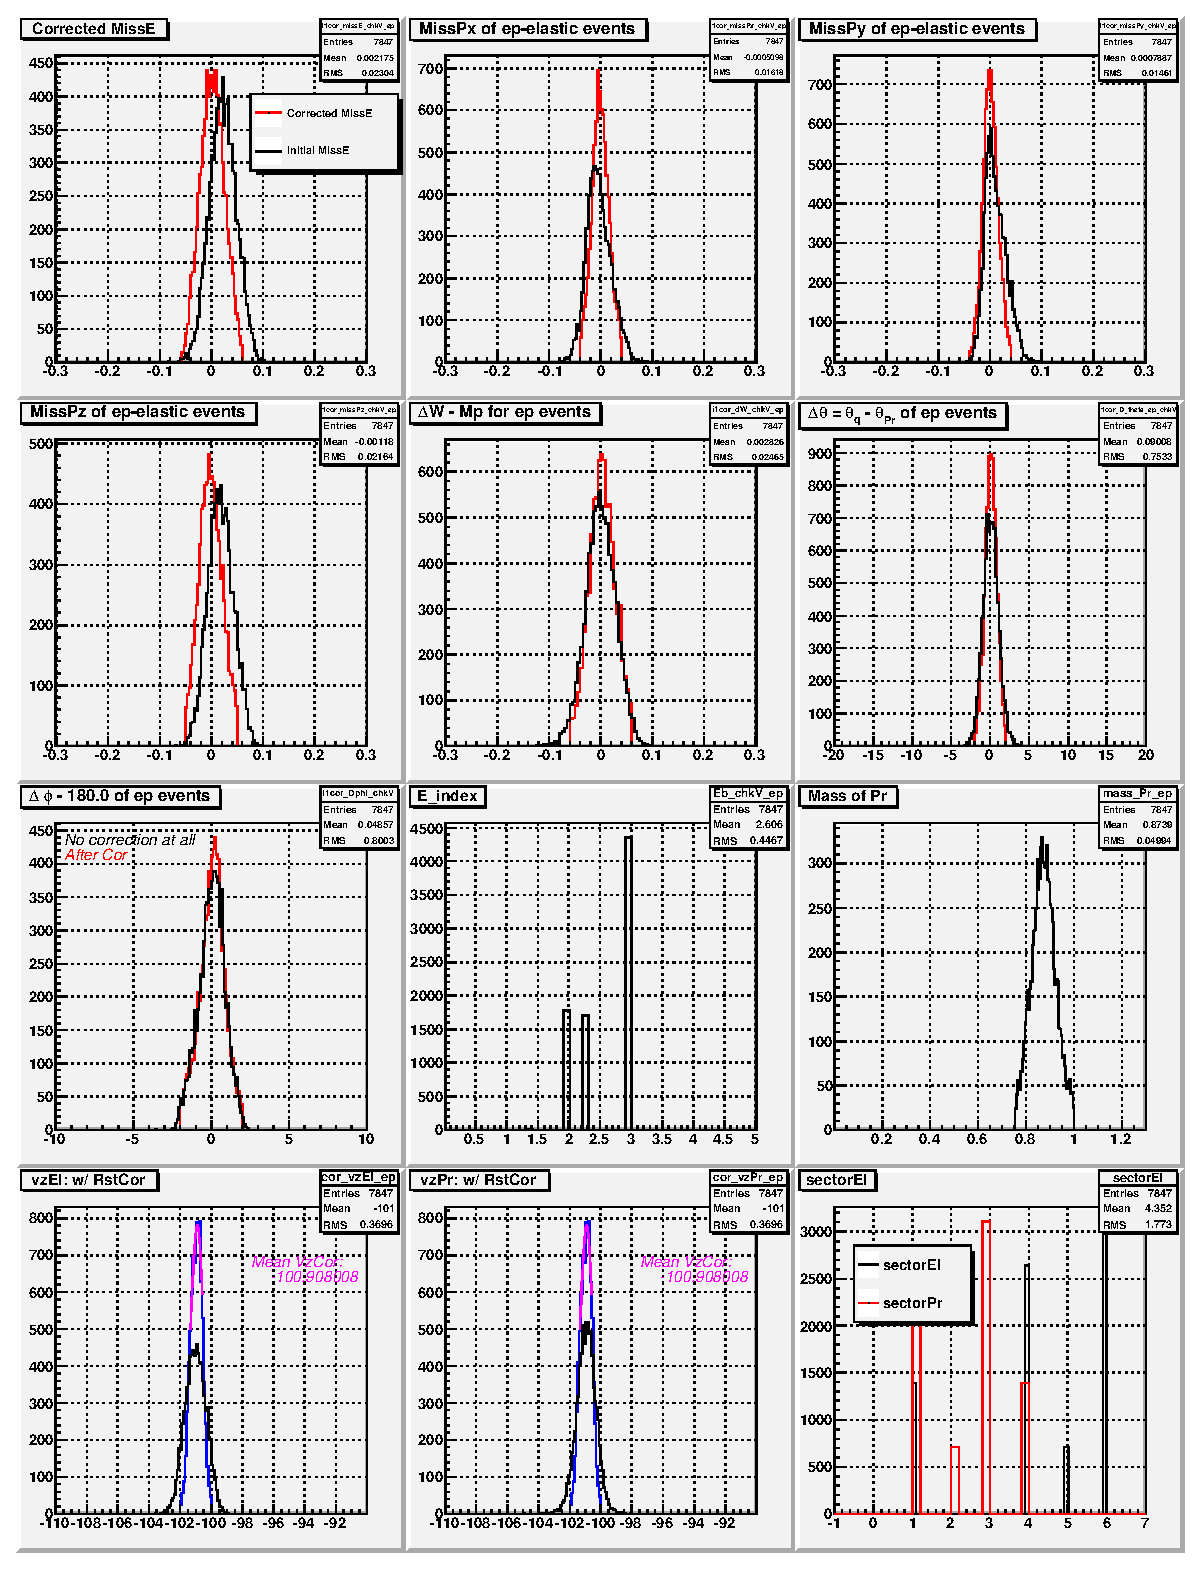
\epsfig{height=20cm,width=15cm,file=chap7KineCor/figures/ep_evntsChkMcor.eps}}
\centering
 \leavevmode 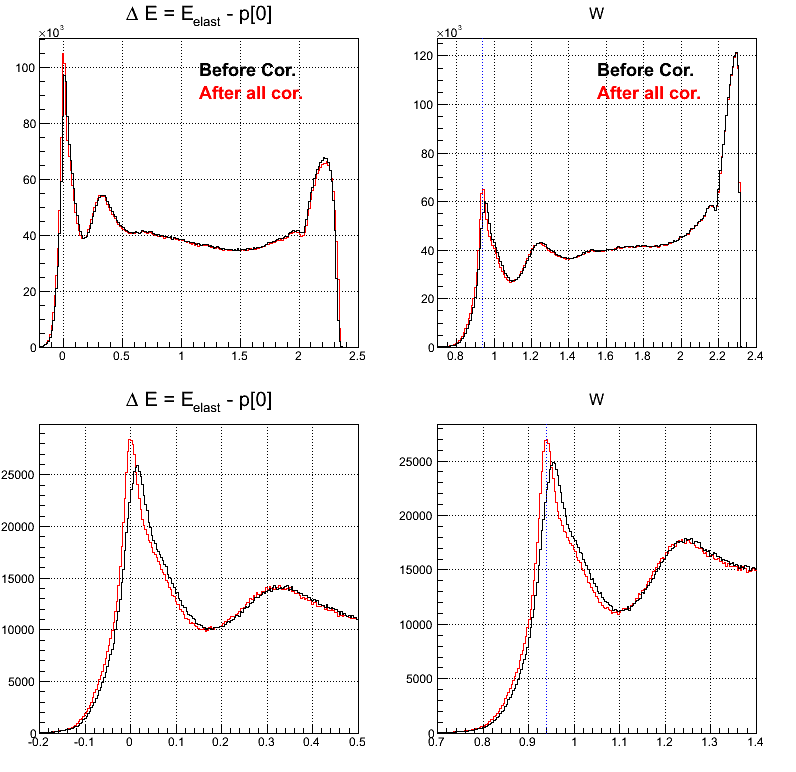
\includegraphics[width=1.0\textwidth]{TexmakerMyFinTh/chap7KineCor/figures/momCorTestInclEi4Pass2Pars11N15_18pTC.png} 
\caption[Effects of corrections on inclusive events from 3 GeV NH$_3$ data]{Effects of kinematic corrections on inclusive events 
from 3 GeV NH$_3$ data. Here, distributions of $\Delta E$ and $W$ are shown in two different ranges. The upper ones shown the full 
range distributions, where as the lower two show the distributions near the quasi-elastic peak. The distributions before the 
corrections are shown by {\bf black continuous} lines and the ones after the corrections are shown by the \textcolor{red}{{\bf red}}% dotted}} 
lines. Here, $E_{elast}$ is the calculated or expected energy of the scattered electron assumming it was scattered off
elastically, whereas, p[0] is the momentum as measured by CLAS.}
\label{fig:epElastic}
\end{figure}
